\lecture{11}{10 Nov.}{}

At the end of \autoref{sec:nibble} we saw that one nibble leaves an uncovered part \(H[V']\) with about \(N e^{-\varepsilon}\) vertices and typical degree about \(D e^{-\varepsilon(r-1)}\). We first check that \(H[V']\) is well-spread again, so that \autoref{lem:nibble} can be applied over and over, and deduce \autoref{thm:pippenger} from it; then we start proving \autoref{lem:nibble}.

\section{Iterating the Nibble}\label{sec:pippenger-proof}

\autoref{lem:nibble} provides some \(\delta = \delta(r,K,\varepsilon,\delta')\), and we may replace it by any smaller \(\delta_{1} \in (0, \delta]\). Indeed, let \(H\) be \((\delta_{1}, K)\)-well-spread with typical degree \(D\). Then \(H\) is also \((\delta, K)\)-well-spread with the same \(D\), because each condition of \autoref{def:well-spread} only gets weaker when \(\delta_{1}\) is raised to \(\delta\):
\[
    \text{(i) } \delta_{1} N \le \delta N \text{ and } (1 \pm \delta_{1}) D \subseteq (1 \pm \delta) D,
    \qquad
    \text{(ii) unchanged},
    \qquad
    \text{(iii) } \operatorname{codeg}(x,y) < \delta_{1} D \le \delta D .
\]
So \autoref{lem:nibble} applies to \(H\) and gives the same conclusions (i)--(iii); that is, the lemma also holds with \(\delta_{1}\) in place of \(\delta\). Taking \(\delta_{1} = \min\{\delta, \delta' e^{-\varepsilon(r-1)}\}\), we may assume from now on that \(\delta \le \delta' e^{-\varepsilon(r-1)}\).

\begin{remark}\label{rmk:nibble-well-spread}
    In \autoref{lem:nibble}, assume \(\delta \le \delta' e^{-\varepsilon(r-1)}\). Then the induced subhypergraph \(H' \coloneqq H[V']\) on \(N' \coloneqq \abs{V'}\) vertices is
    \[
        \bigl( \delta',\, K e^{\varepsilon(r-1)} \bigr)\text{-well-spread with typical degree } D' \coloneqq D e^{-\varepsilon(r-1)} .
    \]
    We check (i)--(iii) of \autoref{def:well-spread} for \(H'\). (i) is exactly (iii) of \autoref{lem:nibble}. Every edge of \(H'\) is an edge of \(H\), so for all \(x, y \in V'\),
    \[
        \begin{aligned}
            \deg_{H'}(x) &\le \deg_{H}(x) < K D = K e^{\varepsilon(r-1)} D', \\
            \operatorname{codeg}_{H'}(x,y) &\le \operatorname{codeg}_{H}(x,y) < \delta D = \delta e^{\varepsilon(r-1)} D' \le \delta' D',
        \end{aligned}
    \]
    which are (ii) and (iii).
\end{remark}

So we can take a nibble from \(H\), then from \(H[V']\), then from what is left after that, and so on. After \(t\) rounds the uncovered set \(V_{t}\) is so small that we can cover each of its vertices by its own edge.
\begin{center}
    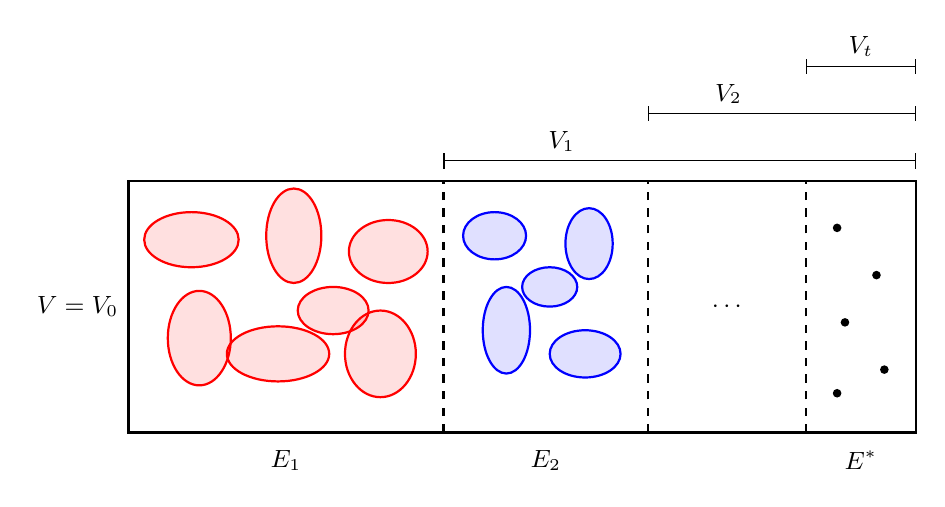
\begin{tikzpicture}[thick, every node/.style={font=\small}, dot/.style={circle, fill, inner sep=1.1pt}, e/.style={draw=#1, fill=#1, fill opacity=0.12}]
        \draw (0,0) rectangle (10,3.2);
        \draw[dashed] (4,0) -- (4,3.2);
        \draw[dashed] (6.6,0) -- (6.6,3.2);
        \draw[dashed] (8.6,0) -- (8.6,3.2);
        % E_1
        \filldraw[e=red] (0.8,2.45) ellipse (0.6 and 0.35);
        \filldraw[e=red] (2.1,2.5) ellipse (0.35 and 0.6);
        \filldraw[e=red] (3.3,2.3) ellipse (0.5 and 0.4);
        \filldraw[e=red] (0.9,1.2) ellipse (0.4 and 0.6);
        \filldraw[e=red] (1.9,1.0) ellipse (0.65 and 0.35);
        \filldraw[e=red] (3.2,1.0) ellipse (0.45 and 0.55);
        \filldraw[e=red] (2.6,1.55) ellipse (0.45 and 0.3);
        % E_2
        \filldraw[e=blue] (4.65,2.5) ellipse (0.4 and 0.3);
        \filldraw[e=blue] (5.85,2.4) ellipse (0.3 and 0.45);
        \filldraw[e=blue] (4.8,1.3) ellipse (0.3 and 0.55);
        \filldraw[e=blue] (5.8,1.0) ellipse (0.45 and 0.3);
        \filldraw[e=blue] (5.35,1.85) ellipse (0.35 and 0.25);
        \node at (7.6,1.6) {\(\cdots\)};
        % V_t
        \foreach \p in {(9.0,2.6),(9.5,2.0),(9.1,1.4),(9.6,0.8),(9.0,0.5)} \node[dot] at \p {};
        % labels
        \node[left] at (0,1.6) {\(V = V_{0}\)};
        \draw[|-|, thin] (4,3.45) -- (10,3.45) node[pos=0.25, above] {\(V_{1}\)};
        \draw[|-|, thin] (6.6,4.05) -- (10,4.05) node[pos=0.3, above] {\(V_{2}\)};
        \draw[|-|, thin] (8.6,4.65) -- (10,4.65) node[midway, above] {\(V_{t}\)};
        \node at (2,-0.35) {\(E_{1}\)};
        \node at (5.3,-0.35) {\(E_{2}\)};
        \node at (9.3,-0.35) {\(E^{*}\)};
    \end{tikzpicture}
\end{center}
The \(i\)-th nibble \(E_{i}\) consists of edges of \(H[V_{i-1}]\), and \(V_{i} = V_{i-1} \setminus \bigcup_{e \in E_{i}} e\) is what it leaves uncovered; \(E^{*}\) covers the vertices of \(V_{t}\) one at a time.

\paragraph{Plan of the proof.} The proof applies \autoref{lem:nibble} \(t\) times in a row, \(H_{0} = H \to H_{1} \to \cdots \to H_{t}\), where \(H_{i} \coloneqq H[V_{i}]\):
\begin{center}
    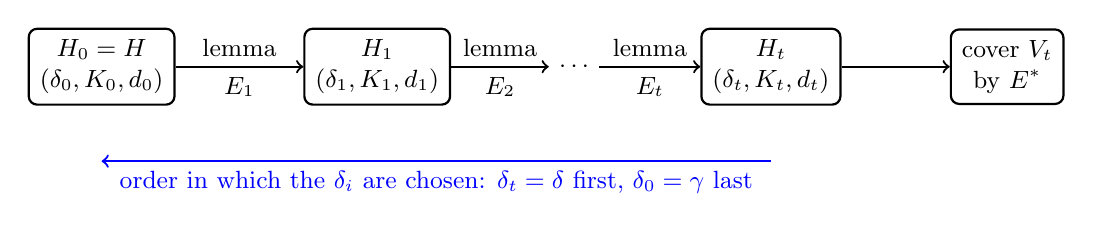
\begin{tikzpicture}[thick, every node/.style={font=\small}, box/.style={draw, rounded corners=3pt, inner sep=4pt, align=center}]
        \node[box] (h0) at (0,0) {\(H_{0} = H\) \\ \((\delta_{0}, K_{0}, d_{0})\)};
        \node[box] (h1) at (3.5,0) {\(H_{1}\) \\ \((\delta_{1}, K_{1}, d_{1})\)};
        \node (dots) at (6.0,0) {\(\cdots\)};
        \node[box] (ht) at (8.5,0) {\(H_{t}\) \\ \((\delta_{t}, K_{t}, d_{t})\)};
        \node[box] (end) at (11.5,0) {cover \(V_{t}\) \\ by \(E^{*}\)};
        \draw[->] (h0) -- node[above] {lemma} node[below] {\(E_{1}\)} (h1);
        \draw[->] (h1) -- node[above] {lemma} node[below] {\(E_{2}\)} (dots);
        \draw[->] (dots) -- node[above] {lemma} node[below] {\(E_{t}\)} (ht);
        \draw[->] (ht) -- (end);
        \draw[->, blue] (8.5,-1.2) -- node[below, align=center] {order in which the \(\delta_{i}\) are chosen: \(\delta_{t} = \delta\) first, \(\delta_{0} = \gamma\) last} (0,-1.2);
    \end{tikzpicture}
\end{center}
Here \((\delta_{i}, K_{i}, d_{i})\) means that \(H_{i}\) is \((\delta_{i}, K_{i})\)-well-spread with typical degree \(d_{i}\). The \(\delta_{i}\) are chosen backwards. We fix \(\delta_{t} = \delta\), the error we want at the end. Then for \(i = t-1, \ldots, 0\) we take \(\delta_{i+1}\) as the \(\delta'\) of \autoref{lem:nibble} and choose \(\delta_{i} \le \delta(r, K_{i}, \varepsilon, \delta_{i+1})\), the input error the lemma needs for that output. The last one chosen, \(\delta_{0}\), is how well-spread \(H\) itself must be, so we take \(\gamma = \delta_{0}\).

\begin{proof}[Proof of \autoref{thm:pippenger} using \autoref{lem:nibble}]
    Fix \(r \ge 2\), \(K \ge 1\) and \(a > 0\).

    \emph{Choosing \(\varepsilon\), \(\delta\), \(t\).} Since \(1 - e^{-\varepsilon} = 1 - \bigl( 1 - \varepsilon + \frac{1}{2}\varepsilon^{2} - \cdots \bigr) = \varepsilon - \frac{1}{2}\varepsilon^{2} + \cdots\), we have \(\frac{\varepsilon}{1 - e^{-\varepsilon}} = \frac{1}{1 - \frac{1}{2}\varepsilon + \cdots} \to 1\) as \(\varepsilon \to 0\). So we can fix \(\varepsilon > 0\) with
    \[
        \frac{\varepsilon}{1 - e^{-\varepsilon}} + r \varepsilon < 1 + a .
    \]
    As this inequality is strict, we can then fix \(0 < \delta < \frac{1}{10}\) with
    \begin{equation}\label{eq:pippenger-delta}
        (1 + 4\delta) \Bigl( \frac{\varepsilon}{1 - e^{-\varepsilon}} + r \varepsilon \Bigr) < 1 + a ,
    \end{equation}
    and \(t \in \mathbb{N}\) with \(e^{-\varepsilon t} < \varepsilon\). \(t\) will be the number of times we apply \autoref{lem:nibble}.

    \emph{Parameters for the lemma, by reverse induction.} Let \(K_{i} \coloneqq K e^{\varepsilon(r-1) i}\) and \(d_{i} \coloneqq D e^{-\varepsilon(r-1) i}\). Start with \(\delta_{t} \coloneqq \delta\) and choose \(\delta_{t-1}, \ldots, \delta_{1}, \delta_{0}\) in this order such that
    \begin{equation}\label{eq:pippenger-deltas}
        \underbrace{\delta_{i} \le \delta_{i+1} e^{-\varepsilon(r-1)}
        \quad\text{and}\quad
        \delta_{i} \le \delta(r, K_{i}, \varepsilon, \delta_{i+1})}_{\text{for each } 0 \le i < t},
        \qquad
        \prod_{j=0}^{t} (1 + \delta_{j}) < 1 + 2\delta .
    \end{equation}
    Here \(\delta(r, K_{i}, \varepsilon, \delta_{i+1})\) is the \(\delta\) of \autoref{lem:nibble} for \(K = K_{i}\) and \(\delta' = \delta_{i+1}\); the product condition holds once \(\delta_{0}, \ldots, \delta_{t-1}\) are small enough. Let \(R_{i} \coloneqq e^{\varepsilon(r-1)i} D_{0}(r, K_{i}, \varepsilon, \delta_{i+1})\). For \(D \ge R_{i}\) we have \(d_{i} \ge D_{0}(r, K_{i}, \varepsilon, \delta_{i+1})\), so we can apply \autoref{lem:nibble} with
    \[
        r, \quad K_{i}, \quad \varepsilon, \quad \delta' = \delta_{i+1}, \quad \delta = \delta_{i}
    \]
    to any \((\delta_{i}, K_{i})\)-well-spread hypergraph with typical degree \(d_{i}\). Finally take \(\gamma \coloneqq \delta_{0}\) and \(D_{0} \coloneqq \max_{i} R_{i}\).

    \emph{Iterating.} Let \(H = (V, E)\) be a \((\gamma, K)\)-well-spread \(r\)-uniform hypergraph on \(N\) vertices with typical degree \(D \ge D_{0}\) and no vertex of degree \(0\). Put \(V_{0} \coloneqq V\). Suppose \(H_{i} \coloneqq H[V_{i}]\) is \((\delta_{i}, K_{i})\)-well-spread with typical degree \(d_{i}\); for \(i = 0\) this is the assumption on \(H\). Applying \autoref{lem:nibble} to \(H_{i}\) with the parameters above gives a set \(E_{i+1}\) of edges of \(H_{i}\) and the uncovered set \(V_{i+1} \coloneqq V_{i} \setminus \bigcup_{e \in E_{i+1}} e\) with
    \begin{equation}\label{eq:pippenger-step}
        \abs{E_{i+1}} = \frac{\varepsilon \abs{V_{i}}}{r} (1 \pm \delta_{i+1}),
        \qquad
        \abs{V_{i+1}} = \abs{V_{i}} e^{-\varepsilon} (1 \pm \delta_{i+1}),
    \end{equation}
    and by \autoref{rmk:nibble-well-spread} (which applies as \(\delta_{i} \le \delta_{i+1} e^{-\varepsilon(r-1)}\)) \(H_{i+1} = H_{i}[V_{i+1}]\) is \((\delta_{i+1}, K_{i} e^{\varepsilon(r-1)}) = (\delta_{i+1}, K_{i+1})\)-well-spread with typical degree \(d_{i} e^{-\varepsilon(r-1)} = d_{i+1}\). So we can apply the lemma \(t\) times and obtain \(E_{1}, \ldots, E_{t}\) and \(V = V_{0} \supseteq V_{1} \supseteq \cdots \supseteq V_{t}\).

    \emph{The cover.} \(E_{i}\) covers \(V_{i-1} \setminus V_{i}\), so \(E_{1} \cup \cdots \cup E_{t}\) covers \(V \setminus V_{t}\). Every vertex has positive degree, so let \(E^{*}\) consist of one edge containing \(x\) for each \(x \in V_{t}\); then \(\abs{E^{*}} \le \abs{V_{t}}\), and
    \[
        E_{1} \cup E_{2} \cup \cdots \cup E_{t} \cup E^{*}
        \quad\text{covers } V, \text{ and has size}\quad
        \le \sum_{i=1}^{t} \abs{E_{i}} + \abs{E^{*}} \le \sum_{i=1}^{t} \abs{E_{i}} + \abs{V_{t}} .
    \]

    \emph{Counting.} By \eqref{eq:pippenger-deltas}, \(\sum_{j} \delta_{j} \le \prod_{j}(1 + \delta_{j}) - 1 < 2\delta\), so \(\prod_{j}(1 - \delta_{j}) \ge 1 - \sum_{j} \delta_{j} > 1 - 2\delta\); hence
    \begin{equation}\label{eq:pippenger-product}
        \prod_{j=1}^{i} (1 \pm \delta_{j}) = 1 \pm 2\delta \qquad\text{for every } i \le t .
    \end{equation}
    Unrolling the second equation of \eqref{eq:pippenger-step} and using \eqref{eq:pippenger-product},
    \[
        \abs{V_{i}} = \abs{V_{i-1}} e^{-\varepsilon} (1 \pm \delta_{i})
        = \abs{V_{i-2}} e^{-2\varepsilon} (1 \pm \delta_{i})(1 \pm \delta_{i-1})
        = \cdots
        = N e^{-i\varepsilon} (1 \pm 2\delta).
    \]
    Then by the first equation of \eqref{eq:pippenger-step}, as \((1 + 2\delta)(1 + \delta_{i}) \le 1 + 3\delta + 2\delta^{2} < 1 + 4\delta\) and \((1 - 2\delta)(1 - \delta_{i}) \ge 1 - 3\delta\),
    \[
        \abs{E_{i}} = \frac{\varepsilon \abs{V_{i-1}}}{r} (1 \pm \delta_{i})
        = \frac{\varepsilon e^{-(i-1)\varepsilon} N}{r} (1 \pm 4\delta).
    \]
    Hence, with \(\sum_{i=1}^{t} e^{-(i-1)\varepsilon} \le \sum_{j \ge 0} e^{-j\varepsilon} = \frac{1}{1 - e^{-\varepsilon}}\) and \(N e^{-t\varepsilon} < \varepsilon N = \frac{N}{r} \cdot r\varepsilon\),
    \[
        \begin{aligned}
            \text{size of cover}
            &\le \sum_{i=1}^{t} \frac{\varepsilon e^{-(i-1)\varepsilon} N}{r} (1 + 4\delta) + N e^{-t\varepsilon} (1 + 2\delta) \\
            &\le \frac{N}{r} \Bigl( \varepsilon \sum_{i=1}^{t} e^{-(i-1)\varepsilon} + r\varepsilon \Bigr) (1 + 4\delta) \\
            &\le \frac{N}{r} \Bigl( \frac{\varepsilon}{1 - e^{-\varepsilon}} + r\varepsilon \Bigr) (1 + 4\delta)
            < (1 + a) \frac{N}{r}
        \end{aligned}
    \]
    by \eqref{eq:pippenger-delta}.
\end{proof}

In the final bound, \(\frac{\varepsilon}{1 - e^{-\varepsilon}} \approx 1 + \frac{\varepsilon}{2}\) is the waste from overlaps inside the nibbles, and \(r\varepsilon\) is the waste from covering the leftover \(V_{t}\) one vertex at a time; both are small when \(\varepsilon\) is.

\section{Proof of the Key Lemma}\label{sec:nibble-lemma-proof}

\begin{recall}[{\autoref{lem:nibble}}]
    For every \(r \ge 2\), \(K \ge 1\), \(\varepsilon > 0\) and \(\delta' > 0\), there are \(\delta = \delta(r,K,\varepsilon,\delta') > 0\) and \(D_0 = D_0(r,K,\varepsilon,\delta')\) such that for every \(N\) and every \(D \ge D_0\) the following holds. If \(H\) is a \((\delta, K)\)-well-spread \(r\)-uniform hypergraph on \(N\) vertices with typical degree \(D\), then there is a set \(E'\) of edges with
    \begin{enumerate}[(i)]
        \item \(\abs{E'} = \frac{\varepsilon N}{r} (1 \pm \delta')\);
        \item the set \(V' \coloneqq V \setminus \bigcup_{e \in E'} e\) of uncovered vertices has \(\abs{V'} = N e^{-\varepsilon} (1 \pm \delta')\);
        \item all but at most \(\delta' \abs{V'}\) vertices of \(V'\) have degree \(D e^{-\varepsilon(r-1)} (1 \pm \delta')\) in the induced hypergraph \(H[V']\).
    \end{enumerate}
\end{recall}

Let \(H = (V, E)\) be a \((\delta, K)\)-well-spread \(r\)-uniform hypergraph on \(N\) vertices with typical degree \(D\). Call \(x\) \vocab{typical} if \(\deg(x) = (1 \pm \delta) D\) and \vocab{atypical} otherwise; by (i) of \autoref{def:well-spread} at most \(\delta N\) vertices are atypical. Below, ``\(D\) large'' also makes \(N\) large: a typical \(x\) lies in at least \((1 - \delta)D\) distinct edges, each of the form \(\{x\} \cup S\) with \(S \in \binom{V \setminus \{x\}}{r-1}\), so \((1 - \delta) D \le \binom{N-1}{r-1} < N^{r-1}\).

Let \(E' \subseteq E\) be a random subset of the edges, where each \(e \in E\) is chosen independently with probability \(\frac{\varepsilon}{D}\). The hypergraph \(H\) is fixed, so \(\abs{E}\) and every \(\deg(x)\) are numbers; the randomness is only in \(E'\), so \(\abs{E'}\), the uncovered set \(V' = V \setminus \bigcup_{e \in E'} e\), \(\abs{V'}\) and the degrees in \(H[V']\) are random variables. 

\emph{Strategy.} We do not fix \(\delta\) and \(D_{0}\) in advance. Keeping \(\delta\) and \(D\) as variables, we find events \(A_{\mathrm{i}}, A_{\mathrm{ii}}, A_{\mathrm{iii}}\), each of probability \(\le 0.01\), such that if none of them occurs, then (i)--(iii) of \autoref{lem:nibble} hold with certain error terms in place of \(\delta'\). These error terms depend only on \(r, K, \varepsilon, \delta, D\), not on \(H\), and tend to \(0\) as \(\delta \to 0\) and \(D \to \infty\). So we can choose \(\delta\) small and \(D_{0}\) large enough that all of them are \(\le \delta'\). Then by the union bound
\[
    \mathbb{P}\bigl( \text{(i), (ii), (iii) all hold} \bigr) \ge 1 - \mathbb{P}(A_{\mathrm{i}} \cup A_{\mathrm{ii}} \cup A_{\mathrm{iii}}) \ge 1 - \bigl( \mathbb{P}(A_{\mathrm{i}}) + \mathbb{P}(A_{\mathrm{ii}}) + \mathbb{P}(A_{\mathrm{iii}}) \bigr) \ge 0.97 > 0 .
\]
An event of positive probability is non-empty, so some subset \(E' \subseteq E\) satisfies (i)--(iii) simultaneously, which is the conclusion of \autoref{lem:nibble}.

\paragraph{(i) The number of chosen edges.} Since \(H\) is \((\delta, K)\)-well-spread, at least \((1 - \delta) N\) vertices have degree \(\ge (1 - \delta) D\), at most \(N\) have degree \(\le (1 + \delta) D\), and the at most \(\delta N\) atypical ones have degree \(< K D\). So the sum of degrees satisfies
\[
    (1 - \delta) N \cdot (1 - \delta) D \le \sum_{x \in V} \deg(x) \le N (1 + \delta) D + \delta N \cdot K D ,
\]
i.e.\ \(\sum_{x \in V} \deg(x) = N D \bigl( 1 \pm f(\delta, K) \bigr)\)
with \(f(\delta, K) \coloneqq (K + 2)\delta\). Each edge is counted \(r\) times in \(\sum_{x} \deg(x)\), so
\[
    \abs{E} = \frac{N D}{r} \bigl( 1 \pm f(\delta, K) \bigr).
\]
The random variable \(\abs{E'} = \sum_{e \in E} \mathbf{1}[e \in E']\) is a sum of \(\abs{E}\) independent \(\operatorname{Ber}\bigl( \frac{\varepsilon}{D} \bigr)\), so \(\abs{E'} \sim \operatorname{Bin}\bigl( \abs{E}, \frac{\varepsilon}{D} \bigr)\), with mean and variance
\[
    \mu \coloneqq \mathbb{E}\bigl[ \abs{E'} \bigr] = \abs{E} \cdot \frac{\varepsilon}{D} = \frac{\varepsilon N}{r} \bigl( 1 \pm f(\delta, K) \bigr),
    \qquad
    \Var\bigl( \abs{E'} \bigr) = \abs{E} \frac{\varepsilon}{D} \Bigl( 1 - \frac{\varepsilon}{D} \Bigr) \le \mu .
\]
\(\mu\) is a number; it remains to show that \(\abs{E'}\) is close to \(\mu\) with high probability. By \thmref{thm:chebyshev} with \(a = \eta \mu\), where \(\eta \coloneqq 10 \mu^{-1/2}\),
\[
    \mathbb{P}\bigl( \abs{\abs{E'} - \mu} \ge \eta \mu \bigr) \le \frac{\Var(\abs{E'})}{\eta^{2} \mu^{2}} \le \frac{1}{\eta^{2} \mu} = 0.01 .
\]
So with probability \(\ge 0.99\),
\[
    \abs{E'} = \mu (1 \pm \eta) = \frac{\varepsilon N}{r} \bigl( 1 \pm f(\delta, K) \bigr)(1 \pm \eta) = \frac{\varepsilon N}{r} (1 \pm \delta^{*}),
    \qquad
    \delta^{*} \coloneqq f(\delta, K) + \eta + f(\delta, K)\, \eta .
\]
Here \(f(\delta, K) = (K+2)\delta \to 0\) as \(\delta \to 0\). Also \(\eta = 10\mu^{-1/2}\) depends on \(H\) only through \(N\), and \(N^{r-1} > (1 - \delta) D\), so \(\eta \to 0\) as \(D \to \infty\). Hence \(\delta^{*} \to 0\) as \(\delta \to 0\) and \(D \to \infty\), and
\[
    \mathbb{P}\Bigl( \abs{E'} = (1 \pm \delta^{*}) \frac{\varepsilon N}{r} \Bigr) \ge 0.99 .
\]
Let \(A_{\mathrm{i}}\) be the complement of this event, so \(\mathbb{P}(A_{\mathrm{i}}) \le 0.01\).

\paragraph{(ii) The number of uncovered vertices.} For every vertex \(x\), let
\[
    I_{x} \coloneqq
    \begin{cases}
        1 & \text{if no edge containing } x \text{ is chosen in } E', \\
        0 & \text{otherwise,}
    \end{cases}
    \qquad\text{so}\qquad
    \abs{V'} = \sum_{x \in V} I_{x} .
\]
The \(\deg(x)\) edges containing \(x\) are chosen independently, so \(\mathbb{E}[I_{x}] = \mathbb{P}(x \text{ is uncovered}) = \bigl( 1 - \frac{\varepsilon}{D} \bigr)^{\deg(x)}\). By linearity of expectation, splitting off the at most \(\delta N\) atypical vertices, each contributing a term in \([0, 1]\),
\[
    \begin{aligned}
        \mathbb{E}\bigl[ \abs{V'} \bigr]
        &= \sum_{x \in V} \Bigl( 1 - \frac{\varepsilon}{D} \Bigr)^{\deg(x)}
        = \sum_{\text{typical } x} \Bigl( 1 - \frac{\varepsilon}{D} \Bigr)^{\deg(x)} \pm \delta N \\
        &= (1 \pm \delta) N \cdot \Bigl( 1 - \frac{\varepsilon}{D} \Bigr)^{(1 \pm \delta) D} \pm \delta N
        = (1 \pm \delta) e^{-(1 \pm \delta)\varepsilon} N \bigl( 1 \pm o(1) \bigr) \pm \delta N ,
    \end{aligned}
\]
using \(\bigl( 1 - \frac{\varepsilon}{D} \bigr)^{D} \to e^{-\varepsilon}\) as \(D \to \infty\). Hence
\begin{equation}\label{eq:nibble-EV}
    \mathbb{E}\bigl[ \abs{V'} \bigr] = e^{-\varepsilon} N \pm g N,
    \qquad\text{where } g \to 0 \text{ as } \delta \to 0,\ D \to \infty .
\end{equation}
For the variance, \(\Var(I_{x}) = \mathbb{E}[I_{x}] - \mathbb{E}[I_{x}]^{2} \le \mathbb{E}[I_{x}]\), so
\[
    \Var\bigl( \abs{V'} \bigr) = \Var\Bigl( \sum_{x} I_{x} \Bigr)
    = \sum_{x} \Var(I_{x}) + \sum_{x \ne y} \Cov(I_{x}, I_{y})
    \le \sum_{x} \mathbb{E}[I_{x}] + \sum_{x \ne y} \bigl( \mathbb{E}[I_{x} I_{y}] - \mathbb{E}[I_{x}] \mathbb{E}[I_{y}] \bigr).
\]
\(I_{x} I_{y} = 1\) iff none of the \(\deg(x) + \deg(y) - \operatorname{codeg}(x,y)\) edges containing \(x\) or \(y\) is chosen. Using \(\operatorname{codeg}(x,y) < \delta D\), and \(\frac{1}{1 - u} \le e^{2u}\), \(e^{u} - 1 \le 2u\) for \(0 \le u \le \frac{1}{2}\),
\[
    \begin{aligned}
        \Var\bigl( \abs{V'} \bigr)
        &\le \mathbb{E}\bigl[ \abs{V'} \bigr] + \sum_{x \ne y} \biggl( \Bigl( 1 - \frac{\varepsilon}{D} \Bigr)^{\deg(x) + \deg(y) - \operatorname{codeg}(x,y)} - \Bigl( 1 - \frac{\varepsilon}{D} \Bigr)^{\deg(x) + \deg(y)} \biggr) \\
        &\le \mathbb{E}\bigl[ \abs{V'} \bigr] + \sum_{x \ne y} \biggl( \Bigl( 1 - \frac{\varepsilon}{D} \Bigr)^{-\operatorname{codeg}(x,y)} - 1 \biggr) \\
        &\le \mathbb{E}\bigl[ \abs{V'} \bigr] + N^{2} \bigl( e^{\frac{2\varepsilon}{D} \cdot \delta D} - 1 \bigr)
        \le N + 4 \varepsilon \delta N^{2} ,
    \end{aligned}
\]
where the second step multiplies the bracket by \(\bigl( 1 - \frac{\varepsilon}{D} \bigr)^{\deg(x) + \deg(y)} \le 1\). So \(\Var(\abs{V'}) = O(\varepsilon \delta N^{2}) + N = o(N^{2})\) as \(\delta \to 0\) and \(N \to \infty\), while \(\mathbb{E}[\abs{V'}]^{2} = \Theta(N^{2})\) by \eqref{eq:nibble-EV}; that is, \(\Var(\abs{V'}) = o\bigl( \mathbb{E}[\abs{V'}]^{2} \bigr)\). By \thmref{thm:chebyshev} with \(a = \eta N\), where \(\eta \coloneqq 10 \bigl( \frac{1}{N} + 4\varepsilon\delta \bigr)^{1/2}\),
\[
    \mathbb{P}\Bigl( \Bigl| \abs{V'} - \mathbb{E}\bigl[ \abs{V'} \bigr] \Bigr| \ge \eta N \Bigr) \le \frac{N + 4\varepsilon\delta N^{2}}{\eta^{2} N^{2}} = 0.01 ,
\]
and with \eqref{eq:nibble-EV}, for the suitable \(\delta^{**} \coloneqq e^{\varepsilon}(g + \eta) \to 0\),
\[
    \mathbb{P}\Bigl( \abs{V'} = e^{-\varepsilon} N (1 \pm \delta^{**}) \Bigr) \ge 0.99 .
\]
Let \(A_{\mathrm{ii}}\) be the complement of this event, so \(\mathbb{P}(A_{\mathrm{ii}}) \le 0.01\).

\paragraph{(iii) Degrees in \(H[V']\).} For \(x \in V\) and an edge \(e \ni x\), let
\[
    F_{x}(e) \coloneqq \{ f \in E : x \notin f,\ e \cap f \ne \varnothing \}
\]
be the edges that meet \(e\) but avoid \(x\).

\begin{definition}[Good vertex]\label{def:good-vertex}
    A vertex \(x\) is \vocab{good} if
    \begin{enumerate}[(G1)]
        \item \(\deg(x) = (1 \pm \delta) D\);
        \item all but at most \(\delta^{1/2} D\) edges \(e\) containing \(x\) satisfy \(\abs{F_{x}(e)} = (1 \pm \delta^{***})(r-1) D\), where \(\delta^{***} \coloneqq (r+2)\delta\).
    \end{enumerate}
\end{definition}

\begin{claim}\label{claim:good-vertices}
    At least \(\bigl( 1 - F(\delta) \bigr) N\) vertices are good, where \(F(\delta) \coloneqq \delta + \delta^{1/2} r K \to 0\) as \(\delta \to 0\).
\end{claim}

\begin{center}
    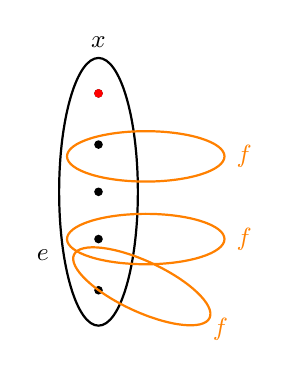
\begin{tikzpicture}[thick, every node/.style={font=\small}, dot/.style={circle, fill, inner sep=1.1pt}]
        \draw (0,0) ellipse (0.5 and 1.7);
        \foreach \y in {1.25,0.6,0,-0.6,-1.25} \node[dot] at (0,\y) {};
        \node[above] at (0,1.7) {\(x\)};
        \node[dot, red] at (0,1.25) {};
        \draw[orange] (0.6,0.45) ellipse (1.0 and 0.32);
        \draw[orange] (0.6,-0.6) ellipse (1.0 and 0.32);
        \draw[orange, rotate around={-25:(0.55,-1.2)}] (0.55,-1.2) ellipse (0.95 and 0.32);
        \node[left] at (-0.5,-0.8) {\(e\)};
        \node[orange] at (1.85,0.45) {\(f\)};
        \node[orange] at (1.85,-0.6) {\(f\)};
        \node[orange] at (1.55,-1.75) {\(f\)};
    \end{tikzpicture}
\end{center}

\begin{proof}
    \emph{Edges through typical vertices only.} Let \(e \ni x\) be such that every \(y \in e \setminus \{x\}\) is typical. With \(A_{y} \coloneqq \{ f \in E : y \in f,\ x \notin f \}\) we have \(F_{x}(e) = \bigcup_{y \in e \setminus \{x\}} A_{y}\) and \(\abs{A_{y}} = \deg(y) - \operatorname{codeg}(x,y)\), while \(\abs{A_{y} \cap A_{z}} \le \operatorname{codeg}(y,z) < \delta D\). By the union bound and by Bonferroni's inequality,
    \[
        \begin{aligned}
            \abs{F_{x}(e)} &\le \sum_{y} \deg(y) \le (r-1)(1 + \delta) D, \\
            \abs{F_{x}(e)} &\ge \sum_{y} \abs{A_{y}} - \sum_{y < z} \abs{A_{y} \cap A_{z}}
            \ge (r-1)(1 - \delta) D - (r-1)\delta D - \tbinom{r-1}{2} \delta D \\
            &\ge (r-1)\bigl( 1 - (r+2)\delta \bigr) D .
        \end{aligned}
    \]
    So an edge \(e \ni x\) violating the condition in (G2) contains an atypical vertex.

    \emph{Counting.} Let \(E_{\mathrm{bad}}\) be the set of edges containing at least one atypical vertex. Each edge of \(E_{\mathrm{bad}}\) contains one of the \(\le \delta N\) atypical vertices, each of which has degree \(< KD\), so
    \[
        \abs{E_{\mathrm{bad}}} \le \underbrace{\delta N}_{\#\text{atypical vertices}} \cdot \underbrace{K D}_{\text{max degree}} .
    \]
    For a vertex \(x\) let \(b(x) \coloneqq \#\{ e \in E_{\mathrm{bad}} : x \in e \}\). Counting the pairs \((x, e)\) with \(e \in E_{\mathrm{bad}}\) and \(x \in e\) once by \(x\) and once by \(e\) (each \(e\) has \(r\) vertices),
    \[
        \sum_{x \in V} b(x) = \sum_{e \in E_{\mathrm{bad}}} \abs{e} = r \abs{E_{\mathrm{bad}}} \le r \delta K N D .
    \]
    If \(x\) violates (G2), then more than \(\delta^{1/2} D\) edges \(e \ni x\) violate the condition in (G2), and each of them lies in \(E_{\mathrm{bad}}\): by \emph{Edges through typical vertices only} above, an edge \(e \ni x\) all of whose other vertices are typical satisfies the condition in (G2), so an edge violating it contains an atypical vertex, so \(b(x) > \delta^{1/2} D\). If \(m\) vertices violate (G2), then \(m \cdot \delta^{1/2} D < \sum_{x} b(x) \le r\delta KND\), so
    \[
        m < \frac{r \delta K N D}{\delta^{1/2} D} = \delta^{1/2} r K N .
    \]
    Hence at most \(\delta N\) vertices violate (G1), at most \(\delta^{1/2} r K N\) vertices violate (G2), and the rest are good.
\end{proof}

\emph{Conditioning on a good \(x \in V'\).} Write \(\deg_{V'}(x)\) for the degree of \(x\) in \(H[V']\). An edge \(e \ni x\) lies in \(H[V']\), and so contributes to \(\deg_{V'}(x)\), iff \(e \subseteq V'\), i.e.\ iff no chosen edge meets \(e\). Given \(x \in V'\), no edge containing \(x\) was chosen, so we need in addition that no edge in
\[
    F_{x}(e) = \{ f : f \not\ni x,\ f \cap e \ne \varnothing \}
\]
was selected.
\begin{center}
    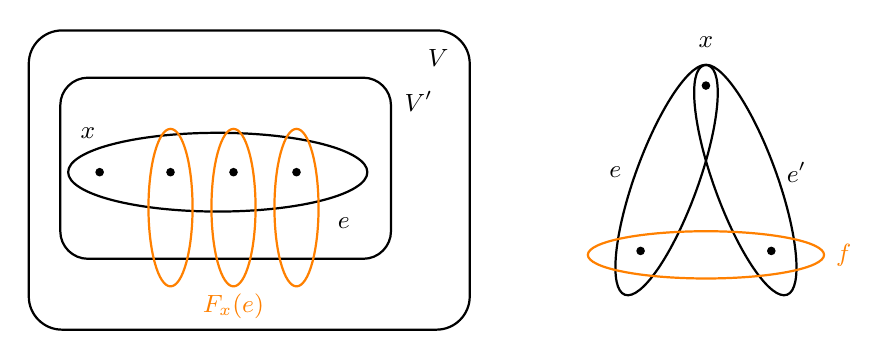
\begin{tikzpicture}[thick, every node/.style={font=\small}, dot/.style={circle, fill, inner sep=1.1pt}]
        \begin{scope}
            \draw[rounded corners=12pt] (0,0) rectangle (5.6,3.8);
            \draw[rounded corners=10pt] (0.4,0.9) rectangle (4.6,3.2);
            \node at (5.2,3.45) {\(V\)};
            \node at (4.95,2.9) {\(V'\)};
            \draw (2.4,2.0) ellipse (1.9 and 0.5);
            \node[dot] at (0.9,2.0) {};
            \foreach \x in {1.8,2.6,3.4} \node[dot] at (\x,2.0) {};
            \node at (0.75,2.5) {\(x\)};
            \node at (4.0,1.35) {\(e\)};
            \foreach \x in {1.8,2.6,3.4} \draw[orange] (\x,1.55) ellipse (0.28 and 1.0);
            \node[orange] at (2.6,0.3) {\(F_{x}(e)\)};
        \end{scope}
        \begin{scope}[xshift=7.4cm, yshift=0.4cm]
            \coordinate (x) at (1.2,2.7);
            \draw[rotate around={70:(0.7,1.5)}] (0.7,1.5) ellipse (1.55 and 0.4);
            \draw[rotate around={-70:(1.7,1.5)}] (1.7,1.5) ellipse (1.55 and 0.4);
            \draw[orange] (1.2,0.55) ellipse (1.5 and 0.3);
            \node[dot] at (x) {};
            \node at (1.2,3.25) {\(x\)};
            \node[dot] at (0.37,0.6) {};
            \node[dot] at (2.03,0.6) {};
            \node at (0.05,1.6) {\(e\)};
            \node at (2.35,1.6) {\(e'\)};
            \node[orange] at (2.95,0.55) {\(f\)};
        \end{scope}
    \end{tikzpicture}
\end{center}
The event \(\{x \in V'\}\) depends only on the edges containing \(x\), which are disjoint from \(F_{x}(e)\), so by independence
\[
    \mathbb{P}\bigl( e \text{ survives} \bigm| x \in V' \bigr) = \Bigl( 1 - \frac{\varepsilon}{D} \Bigr)^{\abs{F_{x}(e)}} .
\]
The lecture ended with the heuristic that this probability is \(\approx e^{-\varepsilon(r-1)}\) for most \(e\); the rest of this section makes it precise and proves (iii).

Write \(p \coloneqq \frac{\varepsilon}{D}\) and \(X_{x} \coloneqq \{x \in V'\}\). Given \(X_{x}\), the edges containing \(x\) are all unchosen and every other edge is still chosen independently with probability \(p\). So with \(Z_{e} \coloneqq \mathbf{1}[e \subseteq V']\) for \(e \ni x\),
\begin{equation}\label{eq:nibble-Ze}
    \deg_{V'}(x) = \sum_{e \ni x} Z_{e},
    \qquad
    \mathbb{P}(Z_{e} = 1 \mid X_{x}) = (1 - p)^{\abs{F_{x}(e)}} .
\end{equation}
Fix a good \(x\). Call \(e \ni x\) \vocab{regular} if \(\abs{F_{x}(e)} = (1 \pm \delta^{***})(r-1)D\). By (G2) all but at most \(\delta^{1/2} D\) edges \(e \ni x\) are regular, and by (G1) \(\deg(x) = (1 \pm \delta) D \le 2D\).

\emph{Conditional expectation.} Since \((1 - \frac{\varepsilon}{D})^{D} \to e^{-\varepsilon}\) as \(D \to \infty\), for regular \(e\)
\[
    (1 - p)^{\abs{F_{x}(e)}} = \Bigl( 1 - \frac{\varepsilon}{D} \Bigr)^{(1 \pm \delta^{***})(r-1)D} = e^{-\varepsilon(r-1)} (1 \pm \theta_{1}),
    \qquad \theta_{1} \to 0 \text{ as } \delta \to 0,\ D \to \infty .
\]
At least \((1 - \delta - \delta^{1/2})D\) and at most \((1 + \delta)D\) edges \(e \ni x\) are regular, and each of the at most \(\delta^{1/2} D\) others contributes a probability in \([0, 1]\) to \eqref{eq:nibble-Ze}. Hence
\[
    \mu_{x} \coloneqq \mathbb{E}\bigl[ \deg_{V'}(x) \bigm| X_{x} \bigr] = D e^{-\varepsilon(r-1)} (1 \pm \theta_{2}),
    \qquad
    \theta_{2} \coloneqq \delta + \theta_{1} + \delta\theta_{1} + \delta^{1/2} e^{\varepsilon(r-1)} .
\]

\emph{Conditional variance.} As in (ii), \(\Var(Z_{e} \mid X_{x}) \le \mathbb{E}[Z_{e} \mid X_{x}]\), and \(Z_{e} Z_{e'} = 1\) iff no edge of \(F_{x}(e) \cup F_{x}(e')\) is chosen, so
\[
    \begin{aligned}
        \Var\bigl( \deg_{V'}(x) \bigm| X_{x} \bigr) &\le \mu_{x} + \sum_{e \ne e' \ni x} \Cov(Z_{e}, Z_{e'} \mid X_{x}), \\
        \Cov(Z_{e}, Z_{e'} \mid X_{x}) &= (1 - p)^{\abs{F_{x}(e) \cup F_{x}(e')}} - (1 - p)^{\abs{F_{x}(e)} + \abs{F_{x}(e')}} \le (1 - p)^{-\abs{F_{x}(e) \cap F_{x}(e')}} - 1 .
    \end{aligned}
\]
This covariance is the dependence in the right figure above. Split the pairs \(e \ne e'\) of edges containing \(x\):
\begin{itemize}
    \item \(\abs{e \cap e'} \ge 2\). Then \(e'\) contains \(x\) and some \(y \in e \setminus \{x\}\), so for each \(e\) there are \(< (r-1)\delta D\) such \(e'\), as \(\operatorname{codeg}(x,y) < \delta D\). There are at most \(2D \cdot r\delta D\) such pairs, each with covariance \(\le 1\).
    \item \(e \cap e' = \{x\}\). An \(f \in F_{x}(e) \cap F_{x}(e')\) contains some \(y \in e \setminus \{x\}\) and some \(z \in e' \setminus \{x\}\) with \(y \ne z\), so \(\abs{F_{x}(e) \cap F_{x}(e')} \le \sum_{y,z} \operatorname{codeg}(y,z) < r^{2}\delta D\). As in (ii), the covariance is \(\le e^{2p \cdot r^{2}\delta D} - 1 \le 4\varepsilon r^{2}\delta\). There are at most \((2D)^{2}\) such pairs.
\end{itemize}
With \(\mu_{x} \le \deg(x) \le 2D\), this gives
\[
    \Var\bigl( \deg_{V'}(x) \bigm| X_{x} \bigr) \le 2D + 2r\delta D^{2} + 16\varepsilon r^{2}\delta D^{2} = \kappa D^{2},
    \qquad
    \kappa \coloneqq \frac{2}{D} + (2r + 16\varepsilon r^{2})\delta .
\]

\emph{Concentration.} \(\mathbb{P}(\,\cdot \mid X_{x})\) is a probability measure, so \thmref{thm:chebyshev} applies to it. With \(a = \theta_{3} D\), where \(\theta_{3} \coloneqq \kappa^{1/3}\),
\[
    \mathbb{P}\bigl( \abs{\deg_{V'}(x) - \mu_{x}} \ge \theta_{3} D \bigm| X_{x} \bigr) \le \frac{\kappa D^{2}}{\theta_{3}^{2} D^{2}} = \theta_{3} .
\]
Otherwise \(\deg_{V'}(x) = \mu_{x} \pm \theta_{3} D = D e^{-\varepsilon(r-1)} (1 \pm \theta_{4})\) with \(\theta_{4} \coloneqq \theta_{2} + \theta_{3} e^{\varepsilon(r-1)}\). Take \(\delta\) and \(D_{0}\) such that \(\theta_{4} \le \delta'\). Then for every good \(x\),
\begin{equation}\label{eq:nibble-good-bad}
    \begin{aligned}
        &\mathbb{P}\Bigl( x \in V' \text{ and } \deg_{V'}(x) \ne D e^{-\varepsilon(r-1)} (1 \pm \delta') \Bigr) \\
        &\qquad = \mathbb{P}(X_{x}) \cdot \mathbb{P}\bigl( \deg_{V'}(x) \ne D e^{-\varepsilon(r-1)} (1 \pm \delta') \bigm| X_{x} \bigr)
        \le \theta_{3} .
    \end{aligned}
\end{equation}

\emph{Counting the exceptions.} Let \(B \coloneqq \{ x \in V' : \deg_{V'}(x) \ne D e^{-\varepsilon(r-1)}(1 \pm \delta') \}\). A vertex of \(B\) is either not good, and by \autoref{claim:good-vertices} there are at most \(F(\delta) N\) of these, or it is good and the event in \eqref{eq:nibble-good-bad} occurs. By linearity of expectation,
\[
    \mathbb{E}\bigl[ \abs{B} \bigr] \le F(\delta) N + \theta_{3} N .
\]
Let \(A_{\mathrm{iii}} \coloneqq \bigl\{ \abs{B} \ge 100 (F(\delta) + \theta_{3}) N \bigr\}\); by \thmref{thm:markov}, \(\mathbb{P}(A_{\mathrm{iii}}) \le 0.01\). If neither \(A_{\mathrm{ii}}\) nor \(A_{\mathrm{iii}}\) occurs, then \(\abs{V'} \ge e^{-\varepsilon} N (1 - \delta^{**}) \ge \frac{1}{2} e^{-\varepsilon} N\) (for \(\delta^{**} \le \frac{1}{2}\)), so
\[
    \abs{B} < 100 \bigl( F(\delta) + \theta_{3} \bigr) N \le 200 e^{\varepsilon} \bigl( F(\delta) + \theta_{3} \bigr) \abs{V'} .
\]
This is (iii) with error \(200 e^{\varepsilon}(F(\delta) + \theta_{3})\) for the number of exceptions and \(\theta_{4}\) for the degrees. Both depend only on \(r, K, \varepsilon, \delta, D\) and tend to \(0\) as \(\delta \to 0\) and \(D \to \infty\), as the Strategy requires. This completes the proof of \autoref{lem:nibble}.
